% Options for packages loaded elsewhere
\PassOptionsToPackage{unicode}{hyperref}
\PassOptionsToPackage{hyphens}{url}
%
\documentclass[
  12pt,
  a4paper,
  DIV=11,
  numbers=noendperiod]{scrreprt}

\usepackage{amsmath,amssymb}
\usepackage{setspace}
\usepackage{iftex}
\ifPDFTeX
  \usepackage[T1]{fontenc}
  \usepackage[utf8]{inputenc}
  \usepackage{textcomp} % provide euro and other symbols
\else % if luatex or xetex
  \usepackage{unicode-math}
  \defaultfontfeatures{Scale=MatchLowercase}
  \defaultfontfeatures[\rmfamily]{Ligatures=TeX,Scale=1}
\fi
\usepackage{lmodern}
\ifPDFTeX\else  
    % xetex/luatex font selection
\fi
% Use upquote if available, for straight quotes in verbatim environments
\IfFileExists{upquote.sty}{\usepackage{upquote}}{}
\IfFileExists{microtype.sty}{% use microtype if available
  \usepackage[]{microtype}
  \UseMicrotypeSet[protrusion]{basicmath} % disable protrusion for tt fonts
}{}
\usepackage{xcolor}
\setlength{\emergencystretch}{3em} % prevent overfull lines
\setcounter{secnumdepth}{5}
% Make \paragraph and \subparagraph free-standing
\ifx\paragraph\undefined\else
  \let\oldparagraph\paragraph
  \renewcommand{\paragraph}[1]{\oldparagraph{#1}\mbox{}}
\fi
\ifx\subparagraph\undefined\else
  \let\oldsubparagraph\subparagraph
  \renewcommand{\subparagraph}[1]{\oldsubparagraph{#1}\mbox{}}
\fi

\usepackage{color}
\usepackage{fancyvrb}
\newcommand{\VerbBar}{|}
\newcommand{\VERB}{\Verb[commandchars=\\\{\}]}
\DefineVerbatimEnvironment{Highlighting}{Verbatim}{commandchars=\\\{\}}
% Add ',fontsize=\small' for more characters per line
\usepackage{framed}
\definecolor{shadecolor}{RGB}{241,243,245}
\newenvironment{Shaded}{\begin{snugshade}}{\end{snugshade}}
\newcommand{\AlertTok}[1]{\textcolor[rgb]{0.68,0.00,0.00}{#1}}
\newcommand{\AnnotationTok}[1]{\textcolor[rgb]{0.37,0.37,0.37}{#1}}
\newcommand{\AttributeTok}[1]{\textcolor[rgb]{0.40,0.45,0.13}{#1}}
\newcommand{\BaseNTok}[1]{\textcolor[rgb]{0.68,0.00,0.00}{#1}}
\newcommand{\BuiltInTok}[1]{\textcolor[rgb]{0.00,0.23,0.31}{#1}}
\newcommand{\CharTok}[1]{\textcolor[rgb]{0.13,0.47,0.30}{#1}}
\newcommand{\CommentTok}[1]{\textcolor[rgb]{0.37,0.37,0.37}{#1}}
\newcommand{\CommentVarTok}[1]{\textcolor[rgb]{0.37,0.37,0.37}{\textit{#1}}}
\newcommand{\ConstantTok}[1]{\textcolor[rgb]{0.56,0.35,0.01}{#1}}
\newcommand{\ControlFlowTok}[1]{\textcolor[rgb]{0.00,0.23,0.31}{#1}}
\newcommand{\DataTypeTok}[1]{\textcolor[rgb]{0.68,0.00,0.00}{#1}}
\newcommand{\DecValTok}[1]{\textcolor[rgb]{0.68,0.00,0.00}{#1}}
\newcommand{\DocumentationTok}[1]{\textcolor[rgb]{0.37,0.37,0.37}{\textit{#1}}}
\newcommand{\ErrorTok}[1]{\textcolor[rgb]{0.68,0.00,0.00}{#1}}
\newcommand{\ExtensionTok}[1]{\textcolor[rgb]{0.00,0.23,0.31}{#1}}
\newcommand{\FloatTok}[1]{\textcolor[rgb]{0.68,0.00,0.00}{#1}}
\newcommand{\FunctionTok}[1]{\textcolor[rgb]{0.28,0.35,0.67}{#1}}
\newcommand{\ImportTok}[1]{\textcolor[rgb]{0.00,0.46,0.62}{#1}}
\newcommand{\InformationTok}[1]{\textcolor[rgb]{0.37,0.37,0.37}{#1}}
\newcommand{\KeywordTok}[1]{\textcolor[rgb]{0.00,0.23,0.31}{#1}}
\newcommand{\NormalTok}[1]{\textcolor[rgb]{0.00,0.23,0.31}{#1}}
\newcommand{\OperatorTok}[1]{\textcolor[rgb]{0.37,0.37,0.37}{#1}}
\newcommand{\OtherTok}[1]{\textcolor[rgb]{0.00,0.23,0.31}{#1}}
\newcommand{\PreprocessorTok}[1]{\textcolor[rgb]{0.68,0.00,0.00}{#1}}
\newcommand{\RegionMarkerTok}[1]{\textcolor[rgb]{0.00,0.23,0.31}{#1}}
\newcommand{\SpecialCharTok}[1]{\textcolor[rgb]{0.37,0.37,0.37}{#1}}
\newcommand{\SpecialStringTok}[1]{\textcolor[rgb]{0.13,0.47,0.30}{#1}}
\newcommand{\StringTok}[1]{\textcolor[rgb]{0.13,0.47,0.30}{#1}}
\newcommand{\VariableTok}[1]{\textcolor[rgb]{0.07,0.07,0.07}{#1}}
\newcommand{\VerbatimStringTok}[1]{\textcolor[rgb]{0.13,0.47,0.30}{#1}}
\newcommand{\WarningTok}[1]{\textcolor[rgb]{0.37,0.37,0.37}{\textit{#1}}}

\providecommand{\tightlist}{%
  \setlength{\itemsep}{0pt}\setlength{\parskip}{0pt}}\usepackage{longtable,booktabs,array}
\usepackage{calc} % for calculating minipage widths
% Correct order of tables after \paragraph or \subparagraph
\usepackage{etoolbox}
\makeatletter
\patchcmd\longtable{\par}{\if@noskipsec\mbox{}\fi\par}{}{}
\makeatother
% Allow footnotes in longtable head/foot
\IfFileExists{footnotehyper.sty}{\usepackage{footnotehyper}}{\usepackage{footnote}}
\makesavenoteenv{longtable}
\usepackage{graphicx}
\makeatletter
\def\maxwidth{\ifdim\Gin@nat@width>\linewidth\linewidth\else\Gin@nat@width\fi}
\def\maxheight{\ifdim\Gin@nat@height>\textheight\textheight\else\Gin@nat@height\fi}
\makeatother
% Scale images if necessary, so that they will not overflow the page
% margins by default, and it is still possible to overwrite the defaults
% using explicit options in \includegraphics[width, height, ...]{}
\setkeys{Gin}{width=\maxwidth,height=\maxheight,keepaspectratio}
% Set default figure placement to htbp
\makeatletter
\def\fps@figure{htbp}
\makeatother

% s\usepackage{juliamono}
\usepackage{indentfirst}
\usepackage{float}
\floatplacement{figure}{H}
\IfFileExists{plex-otf.sty}{
  %% Full TeXlive
  \usepackage[
    % math,
    RM={Scale=0.94},SS={Scale=0.94},SScon={Scale=0.94},TT={Scale=MatchLowercase,FakeStretch=0.9},
    DefaultFeatures={Ligatures=Common}
  ]{plex-otf}
  % \usepackage[Scale=MatchUppercase]{juliamono}
}{
  %% TinyTeX
  \usepackage{libertine}
}
\KOMAoption{captions}{tableheading}
\makeatletter
\@ifpackageloaded{caption}{}{\usepackage{caption}}
\AtBeginDocument{%
\ifdefined\contentsname
  \renewcommand*\contentsname{Содержание}
\else
  \newcommand\contentsname{Содержание}
\fi
\ifdefined\listfigurename
  \renewcommand*\listfigurename{Список иллюстраций}
\else
  \newcommand\listfigurename{Список иллюстраций}
\fi
\ifdefined\listtablename
  \renewcommand*\listtablename{Список таблиц}
\else
  \newcommand\listtablename{Список таблиц}
\fi
\ifdefined\figurename
  \renewcommand*\figurename{Рисунок}
\else
  \newcommand\figurename{Рисунок}
\fi
\ifdefined\tablename
  \renewcommand*\tablename{Таблица}
\else
  \newcommand\tablename{Таблица}
\fi
}
\@ifpackageloaded{float}{}{\usepackage{float}}
\floatstyle{ruled}
\@ifundefined{c@chapter}{\newfloat{codelisting}{h}{lop}}{\newfloat{codelisting}{h}{lop}[chapter]}
\floatname{codelisting}{Список}
\newcommand*\listoflistings{\listof{codelisting}{Листинги}}
\makeatother
\makeatletter
\makeatother
\makeatletter
\@ifpackageloaded{caption}{}{\usepackage{caption}}
\@ifpackageloaded{subcaption}{}{\usepackage{subcaption}}
\makeatother
\ifLuaTeX
\usepackage[bidi=basic]{babel}
\else
\usepackage[bidi=default]{babel}
\fi
\babelprovide[main,import]{russian}
\babelprovide[import]{english}
% get rid of language-specific shorthands (see #6817):
\let\LanguageShortHands\languageshorthands
\def\languageshorthands#1{}
\ifLuaTeX
  \usepackage{selnolig}  % disable illegal ligatures
\fi
\usepackage[style=gost-numeric,backend=biber,langhook=extras,autolang=other*]{biblatex}
\addbibresource{bib/cite.bib}
\usepackage{csquotes}
\usepackage{bookmark}

\IfFileExists{xurl.sty}{\usepackage{xurl}}{} % add URL line breaks if available
\urlstyle{same} % disable monospaced font for URLs
\hypersetup{
  pdftitle={Шаблон отчёта по лабораторной работе},
  pdfauthor={Дмитрий Сергеевич Кулябов},
  pdflang={ru-RU},
  hidelinks,
  pdfcreator={LaTeX via pandoc}}

\title{Шаблон отчёта по лабораторной работе}
\usepackage{etoolbox}
\makeatletter
\providecommand{\subtitle}[1]{% add subtitle to \maketitle
  \apptocmd{\@title}{\par {\large #1 \par}}{}{}
}
\makeatother
\subtitle{Простейший вариант}
\author{Дмитрий Сергеевич Кулябов}
\date{}

\begin{document}
\maketitle

\renewcommand*\contentsname{Содержание}
{
\setcounter{tocdepth}{1}
\tableofcontents
}
\listoffigures
\listoftables
\setstretch{1.5}
\chapter{Цель
работы}\label{ux446ux435ux43bux44c-ux440ux430ux431ux43eux442ux44b}

Здесь приводится формулировка цели лабораторной работы. Формулировки
цели для каждой лабораторной работы приведены в методических указаниях.

Цель данного шаблона --- максимально упростить подготовку отчётов по
лабораторным работам. Модифицируя данный шаблон, студенты смогут без
труда подготовить отчёт по лабораторным работам, а также познакомиться с
основными возможностями разметки Markdown.

\chapter{Задание}\label{ux437ux430ux434ux430ux43dux438ux435}

Здесь приводится описание задания в соответствии с рекомендациями
методического пособия и выданным вариантом.

\chapter{Теоретическое
введение}\label{ux442ux435ux43eux440ux435ux442ux438ux447ux435ux441ux43aux43eux435-ux432ux432ux435ux434ux435ux43dux438ux435}

Здесь описываются теоретические аспекты, связанные с выполнением работы.

Например, в табл.~\ref{tbl-std-dir} приведено краткое описание
стандартных каталогов Unix.

\begin{longtable}[]{@{}
  >{\raggedright\arraybackslash}p{(\columnwidth - 2\tabcolsep) * \real{0.1014}}
  >{\raggedright\arraybackslash}p{(\columnwidth - 2\tabcolsep) * \real{0.8986}}@{}}
\caption{Описание некоторых каталогов файловой системы GNU
Linux}\label{tbl-std-dir}\tabularnewline
\toprule\noalign{}
\begin{minipage}[b]{\linewidth}\raggedright
Имя каталога
\end{minipage} & \begin{minipage}[b]{\linewidth}\raggedright
Описание каталога
\end{minipage} \\
\midrule\noalign{}
\endfirsthead
\toprule\noalign{}
\begin{minipage}[b]{\linewidth}\raggedright
Имя каталога
\end{minipage} & \begin{minipage}[b]{\linewidth}\raggedright
Описание каталога
\end{minipage} \\
\midrule\noalign{}
\endhead
\bottomrule\noalign{}
\endlastfoot
\texttt{/} & Корневая директория, содержащая всю файловую \\
\texttt{/bin} & Основные системные утилиты, необходимые как в
однопользовательском режиме, так и при обычной работе всем
пользователям \\
\texttt{/etc} & Общесистемные конфигурационные файлы и файлы
конфигурации установленных программ \\
\texttt{/home} & Содержит домашние директории пользователей, которые, в
свою очередь, содержат персональные настройки и данные пользователя \\
\texttt{/media} & Точки монтирования для сменных носителей \\
\texttt{/root} & Домашняя директория пользователя \texttt{root} \\
\texttt{/tmp} & Временные файлы \\
\texttt{/usr} & Вторичная иерархия для данных пользователя \\
\end{longtable}

Более подробно про Unix см. в
\autocite{tanenbaum_book_modern-os_ru,robbins_book_bash_en,zarrelli_book_mastering-bash_en,newham_book_learning-bash_en}.

\chapter{Выполнение лабораторной
работы}\label{ux432ux44bux43fux43eux43bux43dux435ux43dux438ux435-ux43bux430ux431ux43eux440ux430ux442ux43eux440ux43dux43eux439-ux440ux430ux431ux43eux442ux44b}

Описываются проведённые действия, в качестве иллюстрации даётся ссылка
на иллюстрацию (рис.~\ref{fig-001}).

\begin{figure}

\centering{

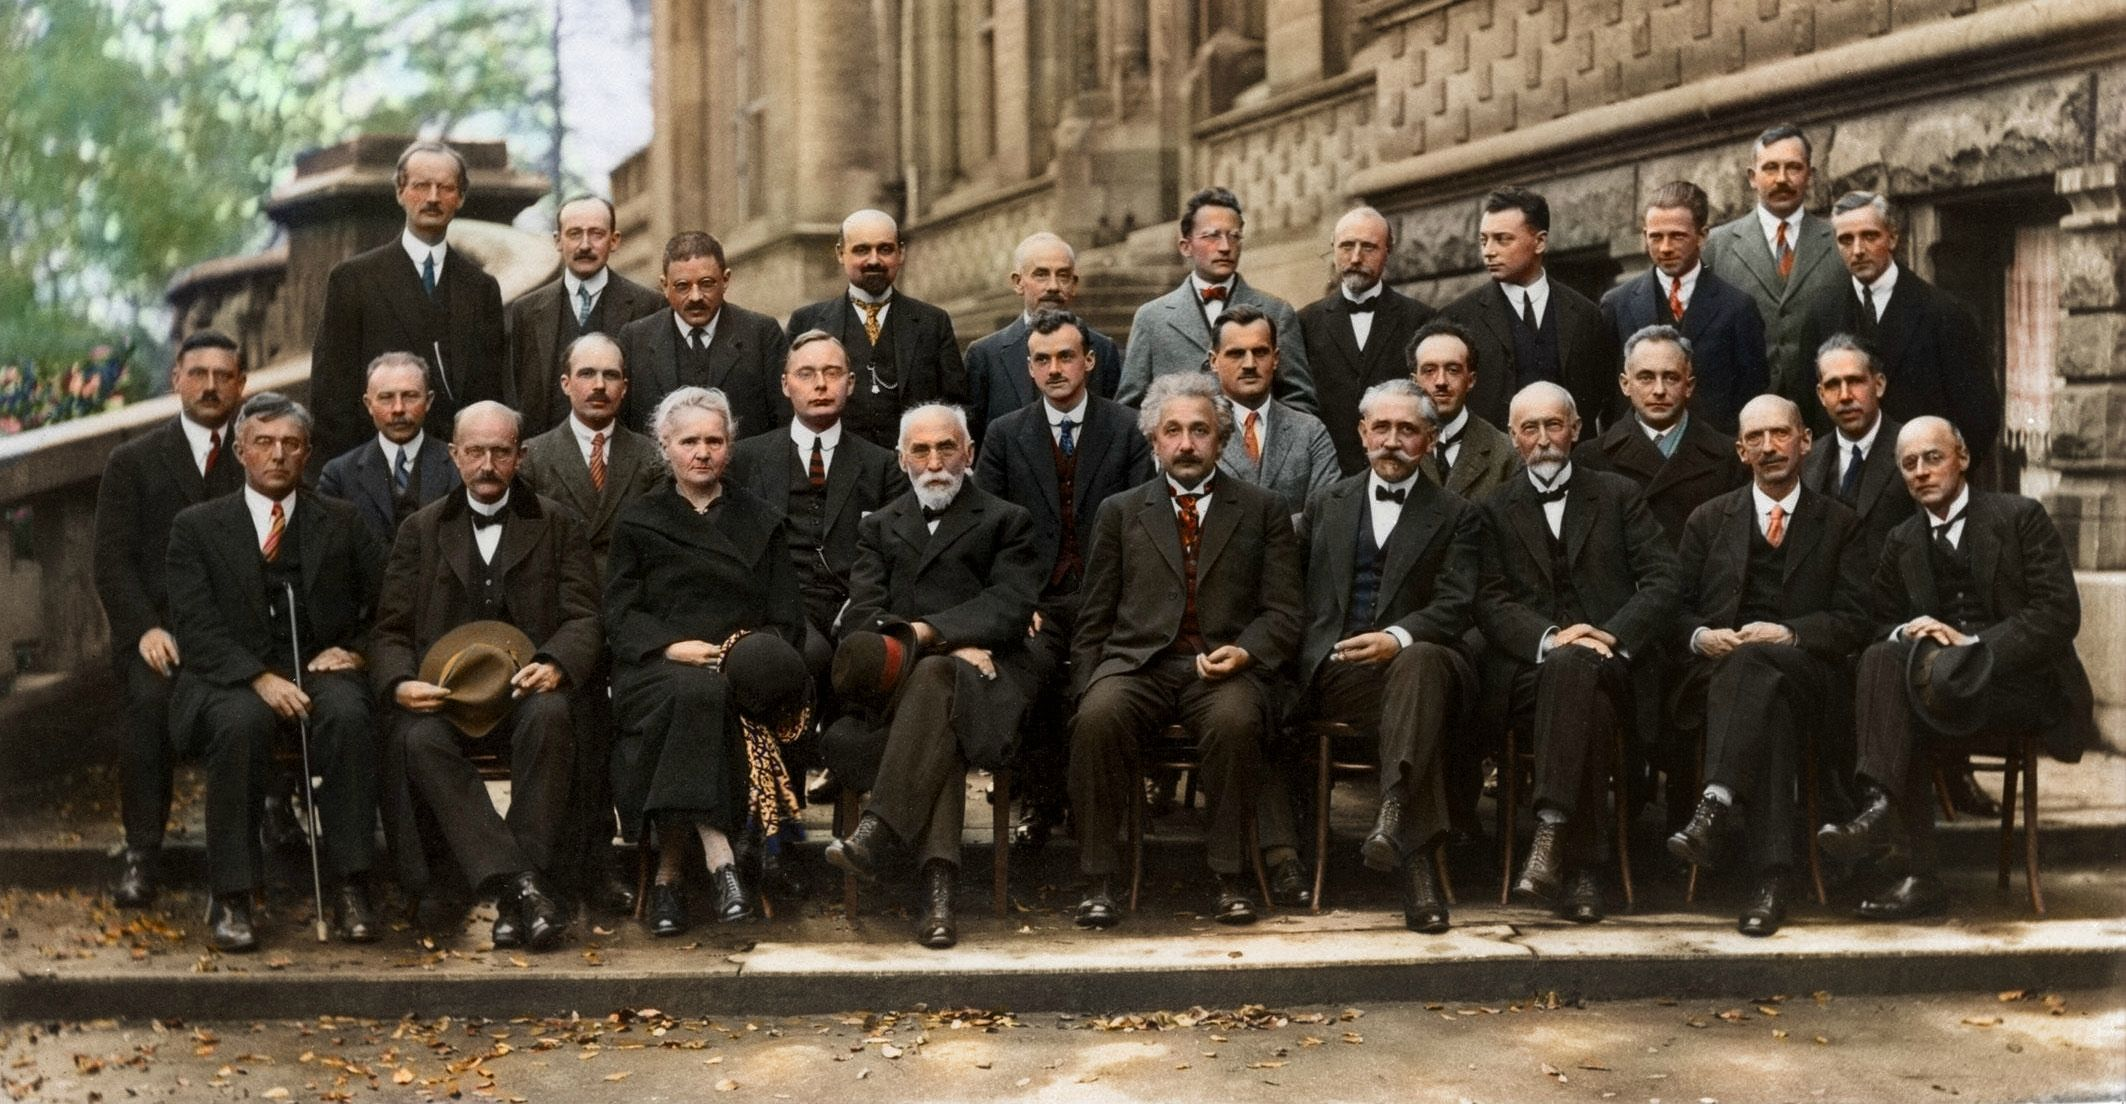
\includegraphics[width=0.7\textwidth,height=\textheight]{image/solvay.jpg}

}

\caption{\label{fig-001}V Сольвеевский конгресс (1927) «Электроны и
фотоны»}

\end{figure}%

\chapter{Экспоненциальный
рост}\label{ux44dux43aux441ux43fux43eux43dux435ux43dux446ux438ux430ux43bux44cux43dux44bux439-ux440ux43eux441ux442}

\textbf{Цель:} Исследовать решение уравнения 𝑑𝑢/𝑑𝑡 = 𝛼𝑢.

\section{Инициализация проекта и загрузка
пакетов}\label{ux438ux43dux438ux446ux438ux430ux43bux438ux437ux430ux446ux438ux44f-ux43fux440ux43eux435ux43aux442ux430-ux438-ux437ux430ux433ux440ux443ux437ux43aux430-ux43fux430ux43aux435ux442ux43eux432}

\begin{Shaded}
\begin{Highlighting}[]
\ImportTok{using} \BuiltInTok{DrWatson}
\PreprocessorTok{@quickactivate} \StringTok{"project"}
\ImportTok{using} \BuiltInTok{DifferentialEquations}
\ImportTok{using} \BuiltInTok{Plots}
\CommentTok{\#force png format}
\FunctionTok{gr}\NormalTok{(size}\OperatorTok{=}\NormalTok{(}\FloatTok{800}\NormalTok{,}\FloatTok{600}\NormalTok{), fmt}\OperatorTok{=:}\NormalTok{png)}
\ImportTok{using} \BuiltInTok{DataFrames}
\ImportTok{using} \BuiltInTok{JLD2}
\NormalTok{script\_name }\OperatorTok{=} \FunctionTok{splitext}\NormalTok{(}\FunctionTok{basename}\NormalTok{(}\ConstantTok{PROGRAM\_FILE}\NormalTok{))[}\FloatTok{1}\NormalTok{]}
\FunctionTok{mkpath}\NormalTok{(}\FunctionTok{plotsdir}\NormalTok{(script\_name))}
\FunctionTok{mkpath}\NormalTok{(}\FunctionTok{datadir}\NormalTok{(script\_name))}
\end{Highlighting}
\end{Shaded}

\begin{verbatim}
┌ Warning: DrWatson could not find find a project file by recursively checking given `dir` and its parents. Returning `nothing` instead.
│ (given dir: /home/nelianjovu)
└ @ DrWatson ~/.julia/packages/DrWatson/2QF5p/src/project_setup.jl:84
\end{verbatim}

\begin{verbatim}
"/home/nelianjovu/work/study/2026-1/2026-1==study--mathmod/2026-1--study--mathmod/labs/lab01/project/data"
\end{verbatim}

\section{Определение
модели}\label{ux43eux43fux440ux435ux434ux435ux43bux435ux43dux438ux435-ux43cux43eux434ux435ux43bux438}

Уравнение экспоненциального роста: 𝑑𝑢/𝑑𝑡 = 𝛼𝑢, 𝑢(0) = 𝑢0

\begin{Shaded}
\begin{Highlighting}[]
\KeywordTok{function} \FunctionTok{exponential\_growth!}\NormalTok{(du, u, p, t)}
\NormalTok{α }\OperatorTok{=}\NormalTok{ p}
\NormalTok{du[}\FloatTok{1}\NormalTok{] }\OperatorTok{=}\NormalTok{ α }\OperatorTok{*}\NormalTok{ u[}\FloatTok{1}\NormalTok{]}
\KeywordTok{end}
\end{Highlighting}
\end{Shaded}

\begin{verbatim}
exponential_growth! (generic function with 1 method)
\end{verbatim}

\section{Первый запуск с параметрами по
умолчанию}\label{ux43fux435ux440ux432ux44bux439-ux437ux430ux43fux443ux441ux43a-ux441-ux43fux430ux440ux430ux43cux435ux442ux440ux430ux43cux438-ux43fux43e-ux443ux43cux43eux43bux447ux430ux43dux438ux44e}

Зададим начальные параметры:

\begin{Shaded}
\begin{Highlighting}[]
\NormalTok{u0 }\OperatorTok{=}\NormalTok{ [}\FloatTok{1.0}\NormalTok{] }\CommentTok{\# начальная популяция}
\NormalTok{α }\OperatorTok{=} \FloatTok{0.3} \CommentTok{\# скорость роста}
\NormalTok{tspan }\OperatorTok{=}\NormalTok{ (}\FloatTok{0.0}\NormalTok{, }\FloatTok{10.0}\NormalTok{) }\CommentTok{\# временной интервал}
\NormalTok{prob }\OperatorTok{=} \FunctionTok{ODEProblem}\NormalTok{(exponential\_growth!, u0, tspan, α)}
\NormalTok{sol }\OperatorTok{=} \FunctionTok{solve}\NormalTok{(prob, }\FunctionTok{Tsit5}\NormalTok{(), saveat}\OperatorTok{=}\FloatTok{0.1}\NormalTok{)}
\end{Highlighting}
\end{Shaded}

\begin{verbatim}
retcode: Success
Interpolation: 1st order linear
t: 101-element Vector{Float64}:
  0.0
  0.1
  0.2
  0.3
  0.4
  0.5
  0.6
  0.7
  0.8
  0.9
  1.0
  1.1
  1.2
  ⋮
  8.9
  9.0
  9.1
  9.2
  9.3
  9.4
  9.5
  9.6
  9.7
  9.8
  9.9
 10.0
u: 101-element Vector{Vector{Float64}}:
 [1.0]
 [1.030454533950446]
 [1.0618365551529674]
 [1.09417430287941]
 [1.1274968605386673]
 [1.161834232745065]
 [1.197217347699063]
 [1.2336780571872568]
 [1.2712491879500347]
 [1.3099646073864084]
 [1.349859018827382]
 [1.3909682733549678]
 [1.433329396499376]
 ⋮
 [14.439892233074882]
 [14.879627505035817]
 [15.332755966505253]
 [15.799688704153079]
 [16.280848966976613]
 [16.776672166300525]
 [17.287605875776944]
 [17.814109831385306]
 [18.356655931432517]
 [18.91572823655281]
 [19.491822969707833]
 [20.085448516186737]
\end{verbatim}

\section{Визуализация
результатов}\label{ux432ux438ux437ux443ux430ux43bux438ux437ux430ux446ux438ux44f-ux440ux435ux437ux443ux43bux44cux442ux430ux442ux43eux432}

Построим график решения:

\begin{Shaded}
\begin{Highlighting}[]
\FunctionTok{plot}\NormalTok{(sol, label}\OperatorTok{=}\StringTok{"u(t)"}\NormalTok{, xlabel}\OperatorTok{=}\StringTok{"Время t"}\NormalTok{, ylabel}\OperatorTok{=}\StringTok{"Популяция u"}\NormalTok{,}
\NormalTok{title}\OperatorTok{=}\StringTok{"Экспоненциальный рост (α = }\SpecialCharTok{$}\StringTok{α)", }\NormalTok{lw}\StringTok{=2, legend=:topleft)}
\end{Highlighting}
\end{Shaded}


\includegraphics{mathmod-lab01-report_files/mediabag/mathmod-lab01-report_files/figure-pdf/cell-6-output-1.pdf}

Сохраним график в папку plots

\begin{Shaded}
\begin{Highlighting}[]
\FunctionTok{savefig}\NormalTok{(}\FunctionTok{plotsdir}\NormalTok{(script\_name, }\StringTok{"exponential\_growth\_α=}\SpecialCharTok{$}\StringTok{α.}\NormalTok{png}\StringTok{"}\NormalTok{))}
\end{Highlighting}
\end{Shaded}

\begin{verbatim}
"/home/nelianjovu/work/study/2026-1/2026-1==study--mathmod/2026-1--study--mathmod/labs/lab01/project/plots/exponential_growth_α=0.3.png"
\end{verbatim}

\section{Анализ
результатов}\label{ux430ux43dux430ux43bux438ux437-ux440ux435ux437ux443ux43bux44cux442ux430ux442ux43eux432}

Создадим таблицу с данными:

\begin{Shaded}
\begin{Highlighting}[]
\NormalTok{df }\OperatorTok{=} \FunctionTok{DataFrame}\NormalTok{(t}\OperatorTok{=}\NormalTok{sol.t, u}\OperatorTok{=}\FunctionTok{first}\NormalTok{.(sol.u))}
\FunctionTok{println}\NormalTok{(}\StringTok{"Первые 5 строк результатов:"}\NormalTok{)}
\FunctionTok{println}\NormalTok{(}\FunctionTok{first}\NormalTok{(df, }\FloatTok{5}\NormalTok{))}
\end{Highlighting}
\end{Shaded}

\begin{verbatim}
Первые 5 строк результатов:
5×2 DataFrame
 Row │ t        u       
     │ Float64  Float64 
─────┼──────────────────
   1 │     0.0  1.0
   2 │     0.1  1.03045
   3 │     0.2  1.06184
   4 │     0.3  1.09417
   5 │     0.4  1.1275
\end{verbatim}

Вычислим удвоение популяции:

\begin{Shaded}
\begin{Highlighting}[]
\NormalTok{u\_final }\OperatorTok{=} \FunctionTok{last}\NormalTok{(sol.u)[}\FloatTok{1}\NormalTok{]}
\NormalTok{doubling\_time }\OperatorTok{=} \FunctionTok{log}\NormalTok{(}\FloatTok{2}\NormalTok{) }\OperatorTok{/}\NormalTok{ α}
\FunctionTok{println}\NormalTok{(}\StringTok{"}\SpecialCharTok{\textbackslash{}n}\StringTok{Аналитическое время удвоения: "}\NormalTok{, }\FunctionTok{round}\NormalTok{(doubling\_time;digits}\OperatorTok{=}\FloatTok{2}\NormalTok{))}
\end{Highlighting}
\end{Shaded}

\begin{verbatim}

Аналитическое время удвоения: 2.31
\end{verbatim}

\section{Сохранение всех
результатов}\label{ux441ux43eux445ux440ux430ux43dux435ux43dux438ux435-ux432ux441ux435ux445-ux440ux435ux437ux443ux43bux44cux442ux430ux442ux43eux432}

\begin{Shaded}
\begin{Highlighting}[]
\PreprocessorTok{@save} \FunctionTok{datadir}\NormalTok{(script\_name, }\StringTok{"all\_results.jld2"}\NormalTok{) df}
\end{Highlighting}
\end{Shaded}

\chapter{Выводы}\label{ux432ux44bux432ux43eux434ux44b}

Здесь кратко описываются итоги проделанной работы.

\chapter*{Список
литературы}\label{ux441ux43fux438ux441ux43eux43a-ux43bux438ux442ux435ux440ux430ux442ux443ux440ux44b}
\addcontentsline{toc}{chapter}{Список литературы}

\printbibliography[heading=none]




\end{document}
